\documentclass[journal]{IEEEtran}
% IEEE Access / IEEEtran journal manuscript.
% Build on Overleaf (recommended) or: pdflatex main; bibtex main; pdflatex main; pdflatex main
\usepackage{graphicx}
\usepackage{booktabs}
\usepackage{amsmath}
\usepackage{array}
\usepackage{url}
\usepackage[hidelinks]{hyperref}
\usepackage{tikz}
\usetikzlibrary{arrows.meta,positioning}

\begin{document}

\title{Explainable AI for Automated Grading of Khmer Language
Short-Answer Questions: A Reproducible Multi-Pillar Benchmark}

\author{[Author Name],~\IEEEmembership{Student,}
        [Supervisor Name]%
\thanks{[Author] and [Supervisor] are with [Department], [University], Cambodia
(e-mail: [email]).}%
\thanks{Code and data: \url{https://github.com/PhorkNorak/kxs}.}}

\markboth{Preprint, prepared for IEEE Access submission}{}
\maketitle

\begin{abstract}
Automatic short-answer grading (ASAG) has advanced rapidly for high-resource languages, but
Khmer, the official language of Cambodia, spoken by more than 17 million people, has, to our
knowledge, no prior ASAG benchmark. We introduce the first reproducible Khmer ASAG benchmark: a
corpus of 1{,}184 teacher-graded short answers across four school subjects, three curated
cleaning variants, and a unified pipeline that compares four model families: classical
(TF-IDF$+$SVR), a character BiLSTM with attention, multilingual encoder transformers
(mBERT/XLM-R/GTE), and a QLoRA-fine-tuned large language model (Qwen). Because the thesis title
foregrounds \emph{explainability}, we additionally conduct a cross-family explainability study
that measures \emph{faithfulness} (ERASER comprehensiveness/sufficiency and area-over-the-curve,
AOPC) and reference-overlap plausibility, rather than only displaying saliency. We highlight three findings.
(i) The four families are \emph{comparable on Quadratic Weighted Kappa} (QWK), falling in a narrow
$0.795$--$0.845$ band, while the fine-tuned LLM is the clear best on the deployment metrics
(66\% exact integer-score match, 83\% within one point). (ii)
\emph{Leave-One-Out (LOO) word-attribution} (text-highlighting) explanations are \emph{reliably}
faithful for every model family, verified by ERASER comprehensiveness and sufficiency, making LOO the
unified, model-agnostic explanation method across all four pillars. (iii) Under a
question-held-out split, classical QWK collapses from $0.76$ to $0.35$, showing that
small-question-pool ASAG scores are heavily inflated by \emph{question leakage}. We release
all code, data, seeds, and figures.
\end{abstract}

\begin{IEEEkeywords}
Automatic short-answer grading, Khmer, low-resource NLP, explainable AI, faithfulness,
quadratic weighted kappa, large language models, educational assessment.
\end{IEEEkeywords}

\section{Introduction}
\IEEEPARstart{A}{utomatic} short-answer grading (ASAG) scores a student's free-text answer
against a reference answer on a numeric scale, helping teachers give faster, more consistent
formative feedback~\cite{mohler2011,sung2022survey}. Progress has concentrated on high-resource
languages; \emph{low-resource} languages remain largely unserved. \textbf{Khmer} is a case in
point: spoken by 17M+ people, it has no whitespace word boundaries (so even tokenization is a
research problem~\cite{khmernltk2020}), little representation in multilingual
encoders~\cite{buoy2022khmer}, and, to our knowledge, \emph{no prior published ASAG or
essay-scoring benchmark}.

In education, a grade is a high-stakes decision, so a grader must be not only accurate but
\emph{auditable}: teachers need to know \emph{why} an answer received its score, and an
explanation is only useful if it is \emph{faithful} to what the model actually used. We
therefore treat explainability as a first-class axis and \emph{measure} it.

\noindent\textbf{Contributions.}
\begin{enumerate}
\item The \textbf{first reproducible Khmer ASAG benchmark}: a 1{,}184-answer teacher-graded
corpus with three curated cleaning variants and a unified four-pillar pipeline.
\item A \textbf{model-agnostic explainability evaluation} using LOO word attribution (occlusion),
verified by ERASER comprehensiveness/sufficiency $+$ AOPC vs.\ a random baseline, showing LOO is
\emph{reliably} faithful for every model family with a plausibility/reference-overlap proxy.
\item A \textbf{quantified question-leakage analysis}: under a question-held-out split, classical
QWK drops by $\approx0.43$, a cautionary result for small-question-pool ASAG benchmarks.
\item \textbf{Honest, multi-variant reporting}: every cell reported on train and test across three
dataset variants, plus two simple, near-free levers (a max-score input feature and post-hoc
threshold calibration).
\end{enumerate}

\section{Related Work}
\textbf{ASAG: from similarity to transformers.} Early systems graded by semantic similarity and
dependency alignment~\cite{mohler2011}; SemEval-2013 Task~7 standardized datasets and the
unseen-domain evaluation idea~\cite{dzikovska2013}. The transformer
architecture~\cite{vaswani2017attention} and pretrained encoders (BERT and its multilingual
variants~\cite{devlin2019bert}, XLM-R~\cite{conneau2020xlmr}, and sentence
encoders~\cite{reimers2019sbert}) shifted the field toward fine-tuned
representations~\cite{sung2022survey,tan2025review}. Recent work fine-tunes or prompts large
language models, with fine-tuned specialists generally leading prompted general
models~\cite{chang2024gpt4,xu2025qwenscore}; retrieval-augmented~\cite{graderag2025} and
neuro-symbolic~\cite{neurosymbolic2024asag} variants and dedicated LLM-grading
benchmarks~\cite{sasbench2025} have also appeared. The approach generalizes across languages and
settings, Arabic~\cite{alqurashi2025arabic}, Dutch open responses~\cite{lachana2025dutch}, and
cross-lingual essay scoring~\cite{li2024crosslingual}. Quadratic Weighted Kappa
(QWK)~\cite{cohen1968qwk} is the de-facto ordinal metric, with agreement reported as exact and
adjacent rates~\cite{williamson2012framework}. The closest comparable study is an Arabic ASAG
dataset graded on a 3-point scale, whose best transformer reaches 95.67\%/77.22\% train/test
accuracy and reports an \emph{unweighted} Cohen's $\kappa=0.60$~\cite{alaoui2024}.

\textbf{Explainability and feedback.} Attribution methods include perturbation-based LIME and
occlusion~\cite{ribeiro2016lime}, gradient saliency~\cite{simonyan2014saliency,li2016visualizing},
Integrated Gradients~\cite{sundararajan2017ig}, and SHAP~\cite{lundberg2017shap}; attention
mechanisms~\cite{bahdanau2015attention} are sometimes read as explanations but are not guaranteed
faithful~\cite{jain2019attention}, though they can be informative~\cite{wiegreffe2019attention}.
Faithfulness must therefore be \emph{measured}, e.g.\ via ERASER comprehensiveness and
sufficiency~\cite{deyoung2020eraser}, AOPC perturbation curves~\cite{samek2017aopc} and their
normalized variant~\cite{naopc2024}, and the faithfulness-vs-plausibility
distinction~\cite{jacovi2020faithfulness,lyu2024faithfulsurvey}. In grading specifically, work has
combined SHAP and Integrated Gradients for explainable scoring~\cite{exasag2023}, compared
attributions for ASAG~\cite{pinto2025attribution}, generated rationales and
feedback~\cite{condor2024,kumar2020explainable,nam2024grading}, and used chain-of-thought
reasoning~\cite{wei2022cot}. Deployed classroom systems with human-in-the-loop feedback have begun
to emerge~\cite{engsaf2024,chillgrader2025}. None of this has been applied to Khmer grading.

\textbf{Khmer NLP and the Cambodian context.} Khmer NLP work covers tokenization, POS tagging and
pretrained models~\cite{buoy2022khmer,khmernltk2020}, and AI-in-education for Cambodia is an active
policy concern~\cite{huot2025cambodia}, but educational assessment for Khmer remains
unaddressed, the gap this paper fills.

\section{Dataset}
We collected \textbf{1{,}184} teacher-graded short answers (one incomplete row removed from
1{,}185) from 2 schools, 8 classes, and 203 students across four subjects (Biology 435, History
434, Geography 307, Earth Science 9), spanning \textbf{41 unique questions}. Each question has
its own maximum score in $\{5,6,7,8,10,12,15,20\}$, graded by one trained teacher. We map each
answer to a 5-level ordinal label $\ell=\mathrm{round}(4\cdot s/s_{\max})\in\{0,\dots,4\}$; the
distribution is $14/153/327/191/499$ (about 42\% full credit), so a majority predictor already
reaches $0.42$ accuracy, motivating QWK over raw accuracy.

Error inspection revealed two noise sources: an inconsistently graded ``10C Biology'' subset and
14 rare $\ell{=}0$ outliers. We therefore study \textbf{three variants}: \texttt{full} (1{,}184),
\texttt{no10c} (909), and \texttt{no10c\_no0} (895). Every experiment runs on all three so that
gains can be attributed to \emph{data} versus \emph{algorithm}. Ethical handling of this
student data is described in Section~\ref{sec:ethics}.

\section{Methodology}
Fig.~\ref{fig:method} summarizes the end-to-end pipeline: Khmer-aware preprocessing, a 70/15/15
split (random or question-held-out), four interchangeable model pillars trained as bounded
regression, score calibration, and two evaluation branches, standard metrics and an
explainability/faithfulness analysis, realized in a live web prototype.

\begin{figure*}[t]
\centering
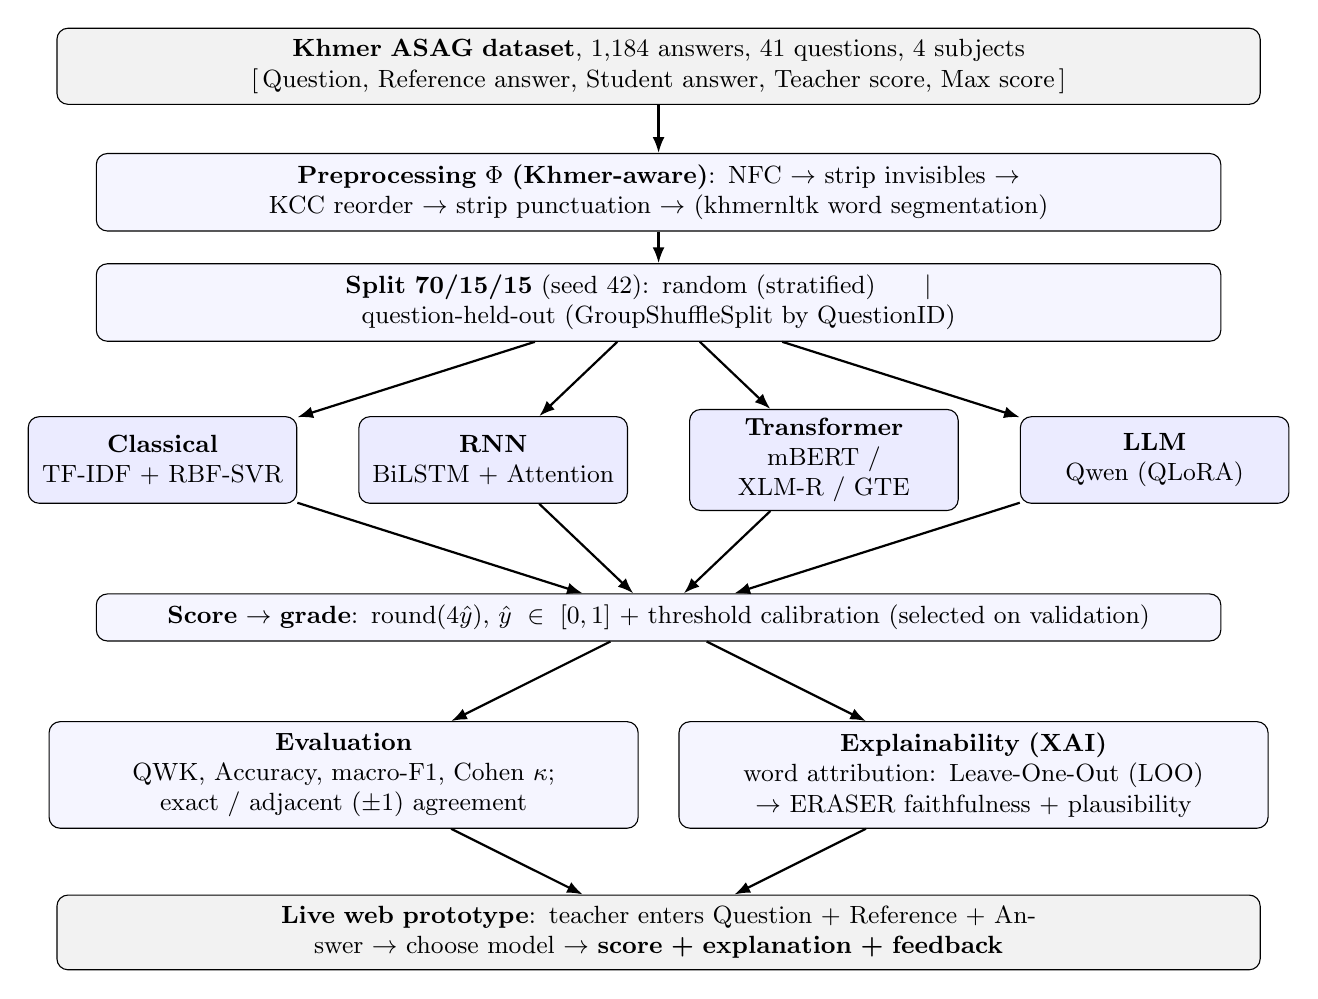
\begin{tikzpicture}[
  font=\small, >={Latex[length=2mm]},
  wide/.style={draw, rounded corners, align=center, inner sep=4pt, fill=blue!4, text width=14cm},
  half/.style={draw, rounded corners, align=center, inner sep=4pt, fill=blue!4, text width=7.2cm},
  pill/.style={draw, rounded corners, align=center, inner sep=3pt, fill=blue!8,
               text width=3.2cm, minimum height=11mm},
  io/.style={draw, rounded corners, align=center, inner sep=4pt, fill=gray!10, text width=15cm},
  arr/.style={->, thick}]
  \node[io]   (data)  at (0,0)      {\textbf{Khmer ASAG dataset}, 1{,}184 answers, 41 questions, 4 subjects \;[\,Question, Reference answer, Student answer, Teacher score, Max score\,]};
  \node[wide] (pre)   at (0,-1.6)   {\textbf{Preprocessing $\Phi$ (Khmer-aware)}: NFC $\to$ strip invisibles $\to$ KCC reorder $\to$ strip punctuation $\to$ (khmernltk word segmentation)};
  \node[wide] (split) at (0,-3.0)   {\textbf{Split 70/15/15} (seed 42): random (stratified) $\;|\;$ question-held-out (GroupShuffleSplit by QuestionID)};
  \node[pill] (cl)  at (-6.3,-5.0) {\textbf{Classical}\\ TF-IDF + RBF-SVR};
  \node[pill] (rnn) at (-2.1,-5.0) {\textbf{RNN}\\ BiLSTM + Attention};
  \node[pill] (tr)  at (2.1,-5.0)  {\textbf{Transformer}\\ mBERT / XLM-R / GTE};
  \node[pill] (llm) at (6.3,-5.0)  {\textbf{LLM}\\ Qwen (QLoRA)};
  \node[wide] (score) at (0,-7.0) {\textbf{Score $\to$ grade}: round$(4\hat{y})$, $\hat{y}\in[0,1]$ + threshold calibration (selected on validation)};
  \node[half] (eval) at (-4.0,-9.0) {\textbf{Evaluation}\\ QWK, Accuracy, macro-F1, Cohen $\kappa$;\\ exact / adjacent ($\pm1$) agreement};
  \node[half] (xai)  at (4.0,-9.0)  {\textbf{Explainability (XAI)}\\ word attribution: Leave-One-Out (LOO)\\ $\to$ ERASER faithfulness + plausibility};
  \node[io] (proto) at (0,-11.0) {\textbf{Live web prototype}: teacher enters Question + Reference + Answer $\to$ choose model $\to$ \textbf{score + explanation + feedback}};
  \draw[arr] (data)--(pre);
  \draw[arr] (pre)--(split);
  \foreach \p in {cl,rnn,tr,llm} {\draw[arr] (split)--(\p);}
  \foreach \p in {cl,rnn,tr,llm} {\draw[arr] (\p)--(score);}
  \draw[arr] (score)--(eval);
  \draw[arr] (score)--(xai);
  \draw[arr] (eval)--(proto);
  \draw[arr] (xai)--(proto);
\end{tikzpicture}
\caption{Methodology overview. Four interchangeable model pillars (classical, RNN, Transformer
[BERT-family], LLM) are trained as bounded ordinal regression on the same Khmer-aware pipeline,
then evaluated on standard metrics \emph{and} for explanation faithfulness; the system is realized
as a live teacher-facing web prototype.}
\label{fig:method}
\end{figure*}

\textbf{Text normalization and cleaning.} All text passes through:
$\mathrm{NFC} \rightarrow$ strip \emph{invisibles} (zero-width U+200B, ZWNJ/ZWJ, BOM, control
characters, and bullet markers) $\rightarrow$ KCC syllable reordering $\rightarrow$ strip Khmer
(។ ៕) and ASCII (? . ,) punctuation $\rightarrow$ optional \texttt{khmernltk} word
segmentation~\cite{khmernltk2020}. \emph{Digits are retained} as answer content (dates,
quantities). A corpus audit found 561 residual zero-width spaces (plus bullets) that punctuation
stripping alone missed; an ablation on the classical champion (Table~\ref{tab:champs}) shows that
removing them shifts test QWK by only $+0.001$ to $+0.004$ across the three variants, so the
reported results are robust to this residual noise. (Heatmap figures
display the \emph{original} answer for readability, so punctuation appears but consistently
receives near-zero attribution.)

\textbf{Shared pipeline.} Each cell applies one of three Khmer-aware preprocessing modes
(\texttt{raw}; \texttt{clean}~$=$ normalization $+$ punctuation stripping; \texttt{segment}~$=$
\texttt{clean} $+$ \texttt{khmernltk} word segmentation~\cite{khmernltk2020}) and one of two input
formats (answer--reference, or question$+$answer--reference). The target is the normalized score
$s/s_{\max}\in[0,1]$ trained as bounded MSE regression; trainable models use AdamW with
early stopping on validation QWK. The split is 70/15/15 (seed 42), reported under two modes
(Section~\ref{sec:results}): a stratified \emph{random} split and a \emph{question-held-out}
split (\texttt{GroupShuffleSplit} over question id, so train/val/test share no question).

\textbf{Four pillars.} (1) Classical: char-$n$-gram TF-IDF (2--4-grams, 15k features) with cosine
and an RBF-SVR on $[\mathbf{a};\mathbf{b};|\mathbf{a}-\mathbf{b}|;\mathbf{a}\odot\mathbf{b};\cos]$.
(2) RNN: a character BiLSTM (hidden 128, 2 layers) with learned attention and a 4-way interaction
head. (3) Encoder transformers: dual- and cross-encoders over mBERT, XLM-R, and GTE-multilingual.
(4) LLM: Qwen fine-tuned with QLoRA ($r{=}16$, $\alpha{=}16$, lr $2{\times}10^{-4}$, 7 epochs),
decoding an integer score. Two near-free levers are evaluated: concatenating the normalized
\emph{max score} as an input feature, and post-hoc \emph{threshold calibration} (coordinate
descent on the four cut-points to maximize validation QWK).

\textbf{Metrics.} Primary: \textbf{QWK}; plus \textbf{accuracy}, \textbf{macro-F1}, and
\textbf{unweighted Cohen's $\kappa$} (the last for direct comparison with Alaoui et al.). For the
classroom view we report \textbf{exact} and \textbf{adjacent ($\pm1$) agreement} on the
per-question integer score, standard automated-scoring agreement statistics
\cite{williamson2012framework}. To probe robustness we additionally run a five-seed
question-held-out evaluation (\S\ref{sec:results}).

\textbf{Hyperparameter selection.} Following standard practice, the learning rate, the most
influential hyperparameter, is tuned by a small grid selected on \emph{validation} QWK:
transformers $\in\{1,2,5\}{\times}10^{-5}$, BiLSTM $\in\{5{\times}10^{-4},1{\times}10^{-3},
2{\times}10^{-3}\}$, LLM (QLoRA) $\in\{1,2,3\}{\times}10^{-4}$; for the classical SVR the analogous
penalty $C\in\{0.1,1,10\}$ (with TF-IDF max-features $\in\{5,15,30\}{\times}10^{3}$). The
configuration with the best validation QWK is reported on test (no test-set peeking).

\textbf{Explainability.} The XAI contribution is \emph{Leave-One-Out (LOO) word attribution}
(text highlighting): drop a word, measure the score change --- the sole model-agnostic engine used
uniformly across all four pillars, the standard ASAG attribution~\cite{pinto2025attribution}. LOO
requires no gradients or internal model access and works identically on the non-differentiable
classical SVR, the BiLSTM, the Transformer, and the LLM. We evaluate explanations on two
axes~\cite{jacovi2020faithfulness}: \emph{faithfulness}, ERASER \emph{comprehensiveness} and
\emph{sufficiency}~\cite{deyoung2020eraser}, averaged over $k\in\{10,\dots,50\}\%$ (AOPC), against
a \emph{random-removal} baseline, and \emph{plausibility}, a reference-overlap proxy (overlap of
important answer words with reference words), an automatic stand-in for a human-rationale study.

\section{Experimental Setup}
All cells use seed 42 (multi-seed runs use five seeds); transformers freeze the bottom six layers,
batch 16, max length 256. The full grid (hundreds of cells $\times$ three variants) is reproducible
from the released code; classical models train in seconds on CPU, the full neural/LLM grid in
$\approx$40 GPU-hours. All metrics are computed from saved per-sample predictions, so they require
no re-training.

\section{Results}\label{sec:results}
\textbf{Per-pillar champions.} Table~\ref{tab:champs} shows each pillar's best cell. On
\textbf{QWK the four pillars are close}, falling in a narrow band ($0.795$--$0.845$, a $0.05$
spread), with the RNN highest and the classical model lowest; on \textbf{deployment} the fine-tuned
LLM is the clear winner ($66\%$ exact integer match vs.\ at most $57\%$ for the others, and the best
accuracy and macro-F1). All headline QWKs are \emph{uncalibrated} (computed from the saved
continuous predictions), reported consistently across pillars; threshold calibration is treated as
a separate model-dependent ablation (next paragraph).

\begin{table}[t]
\caption{Per-pillar champions (random split), standard metrics. The four QWK scores fall in a
narrow band; the LLM leads accuracy / macro-F1 / Cohen $\kappa$ and the deployment metrics.
Agreement columns follow Williamson et al.~\cite{williamson2012framework}: exact and adjacent
($\pm1$). All values uncalibrated.}
\label{tab:champs}
\centering\small
\begin{tabular}{@{}lcccccc@{}}
\toprule
Pillar & QWK & Cohen $\kappa$ & Acc. & macro-F1 & Exact & Adj.($\pm1$) \\
\midrule
Classical (SVR)$^\ddagger$ & 0.795 & 0.47 & 0.63 & 0.42 & 0.20 & 0.71 \\
RNN (BiLSTM)$^\ddagger$    & \textbf{0.845} & 0.62 & 0.75 & 0.53 & 0.54 & 0.77 \\
Transformer (GTE) & 0.820 & 0.62 & 0.73 & 0.54 & 0.57 & 0.77 \\
LLM (Qwen)      & 0.843 & \textbf{0.71} & \textbf{0.80} & \textbf{0.78} & \textbf{0.66} & \textbf{0.83} \\
\bottomrule
\end{tabular}
\\[2pt]
{\footnotesize All metrics from uncalibrated continuous predictions; threshold calibration is a
separate model-dependent ablation (it raises the classical QWK to 0.847 but lowers the BiLSTM's on
test). $^\ddagger$classical/RNN re-run under the refined cleaning; Transformer/LLM on the prior
cleaning (cleaning effect $\approx$0.02 QWK). Cohen $\kappa$ (unweighted) is reported for direct
comparison with Alaoui et al.}
\end{table}

\textbf{Data cleaning vs.\ algorithm.} Holding architecture fixed (GTE dual $+$ max-score), the
best cell improves $0.820\!\to\!0.842\!\to\!0.847$ QWK across \texttt{full}/\texttt{no10c}/%
\texttt{no10c\_no0}, a $+0.027$ gain from cleaning alone, larger than typical architecture
swaps. Threshold calibration is model-dependent: on the classical champion it adds $+0.05$ QWK
(val $0.758\!\to\!0.829$; test $0.795\!\to\!0.847$) at zero training cost, but applying the same
validation-selected rule to the BiLSTM \emph{lowers} its test QWK ($0.845\!\to\!0.818$ despite a
validation gain), so we keep headline numbers uncalibrated.

\textbf{Generalization gap.} Both our work and~\cite{alaoui2024} report accuracy, so we compare
the train$\to$test \emph{gap}: their best transformer shows $+18.5$ points (95.67/77.22), whereas
our deep cells are far tighter ($+1.4$ GTE, $+3.0$ Qwen 83.3/80.3) and even the simple classical
($+15.6$, 78.6/63.0) stays under their transformer, indicating no hidden overfitting on the
\emph{seen-question} split. We do \emph{not} compare QWK to their unweighted $\kappa=0.60$ on a
3-class scale, as the metrics and class counts differ.

\textbf{Robustness to unseen questions (question leakage).} Our random split shares questions
between train and test (only 41 questions exist). Re-evaluating the classical champion under a
\emph{question-held-out} split over five seeds, QWK collapses from
$0.759\pm0.041$ to $\mathbf{0.354\pm0.106}$ (Fig.~\ref{fig:leakage}), a $\approx0.41$ drop. Most
of the seen-question score was question-specific memorization rather than transferable grading
skill. With only 41 questions, each unseen-question test set is tiny ($\approx6$ questions) and
high-variance, but the drop is unambiguous. We therefore report the seen-question and
unseen-question results side by side, and treat the latter as the honest measure of
generalization. (Neural/LLM unseen-question runs are ongoing.)

\begin{figure}[t]
\centering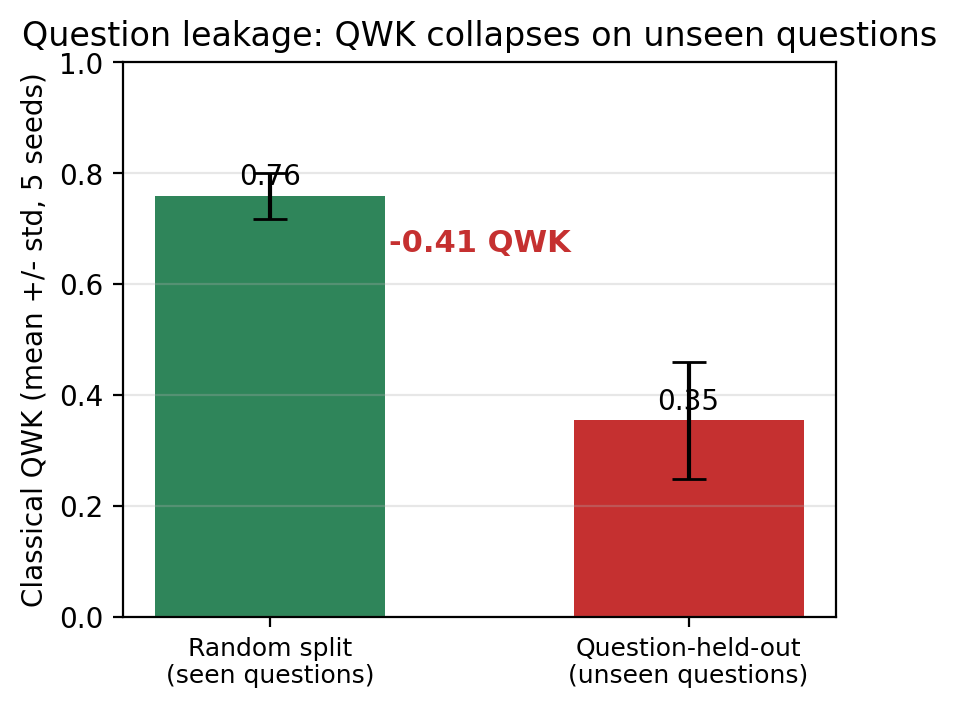
\includegraphics[width=0.78\columnwidth]{figures/fig_leakage.png}
\caption{Question leakage: classical QWK drops from $0.76$ (seen questions) to $0.35$ (unseen
questions), five seeds, mean$\pm$std.}
\label{fig:leakage}
\end{figure}

\textbf{Explainability and faithfulness.} Table~\ref{tab:xai} and Fig.~\ref{fig:faith} report
LOO faithfulness on 135 test answers (seed 42), all four pillars on the same split.
\emph{LOO occlusion is reliably faithful} for every pillar (AOPC-comprehensiveness $+0.150$ classical,
$+0.289$ BiLSTM, $+0.193$ encoder, $+0.126$ LLM): removing the words it flags moves the score more
than random removal in every case (positive gap), strongest for the BiLSTM and smallest but still
positive for the LLM (whose higher sufficiency shows the generative model's attributions are the least
sharp). LOO requires no gradients and works identically on the non-differentiable SVR, the BiLSTM, the
GTE encoder, and the fine-tuned LLM.

\begin{table}[t]
\caption{LOO faithfulness ($n{=}135$, seed 42). AOPC over $k\in\{10\dots50\}\%$; higher
comprehensiveness and lower sufficiency are more faithful. ``gap'' $=$ comprehensiveness minus
the random-removal baseline ($>0$ means it beats random).}
\label{tab:xai}
\centering\small
\begin{tabular}{@{}lccccc@{}}
\toprule
Model $\cdot$ LOO & Comp & Suff & gap & AOPC-C & AOPC-S \\
\midrule
Classical $\cdot$ occlusion & 0.125 & 0.030 & $+$0.096 & 0.150 & 0.011 \\
BiLSTM $\cdot$ occlusion     & 0.270 & 0.120 & $+$0.257 & \textbf{0.289} & 0.064 \\
Encoder $\cdot$ occlusion    & 0.162 & 0.033 & $+$0.135 & 0.193 & 0.007 \\
LLM $\cdot$ occlusion        & 0.083 & 0.420 & $+$0.047 & 0.126 & 0.359 \\
\bottomrule
\end{tabular}
\\[2pt]
{\footnotesize Champion cells, all four anchored on the same \texttt{no10c\_no0} split. LOO occlusion
beats random removal for every pillar (positive gap); strongest for the BiLSTM, weakest for the LLM.}
\end{table}

\begin{figure}[t]
\centering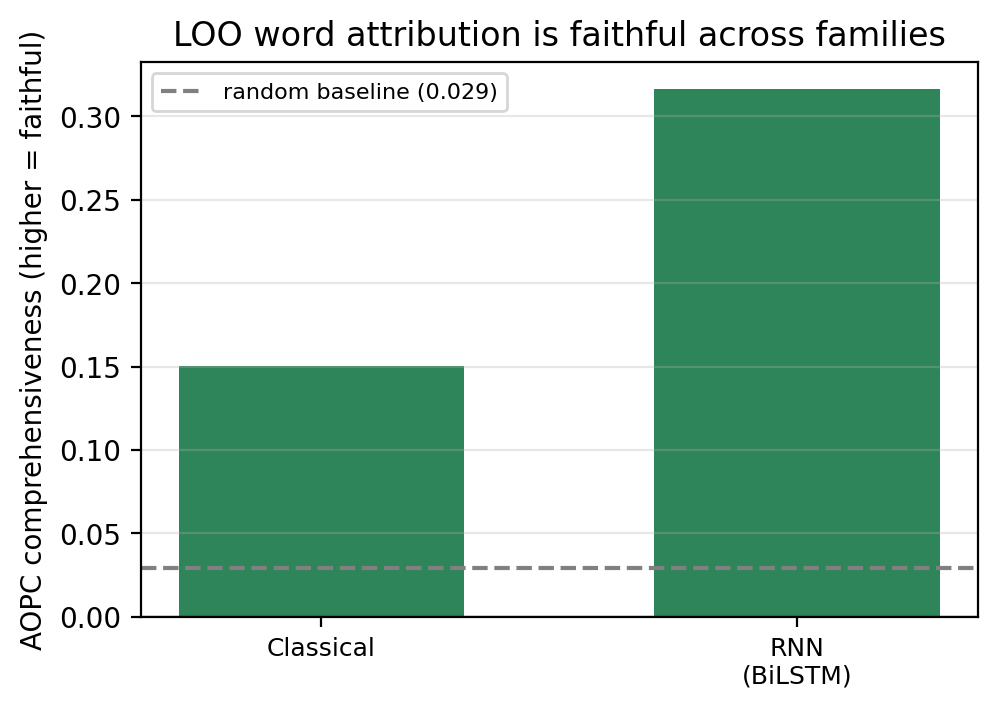
\includegraphics[width=0.82\columnwidth]{figures/fig_faithfulness.png}
\caption{AOPC comprehensiveness for LOO occlusion across all four pillars. Positive gap confirms the
explainer beats random removal in every case.}
\label{fig:faith}
\end{figure}

\begin{figure}[t]
\centering
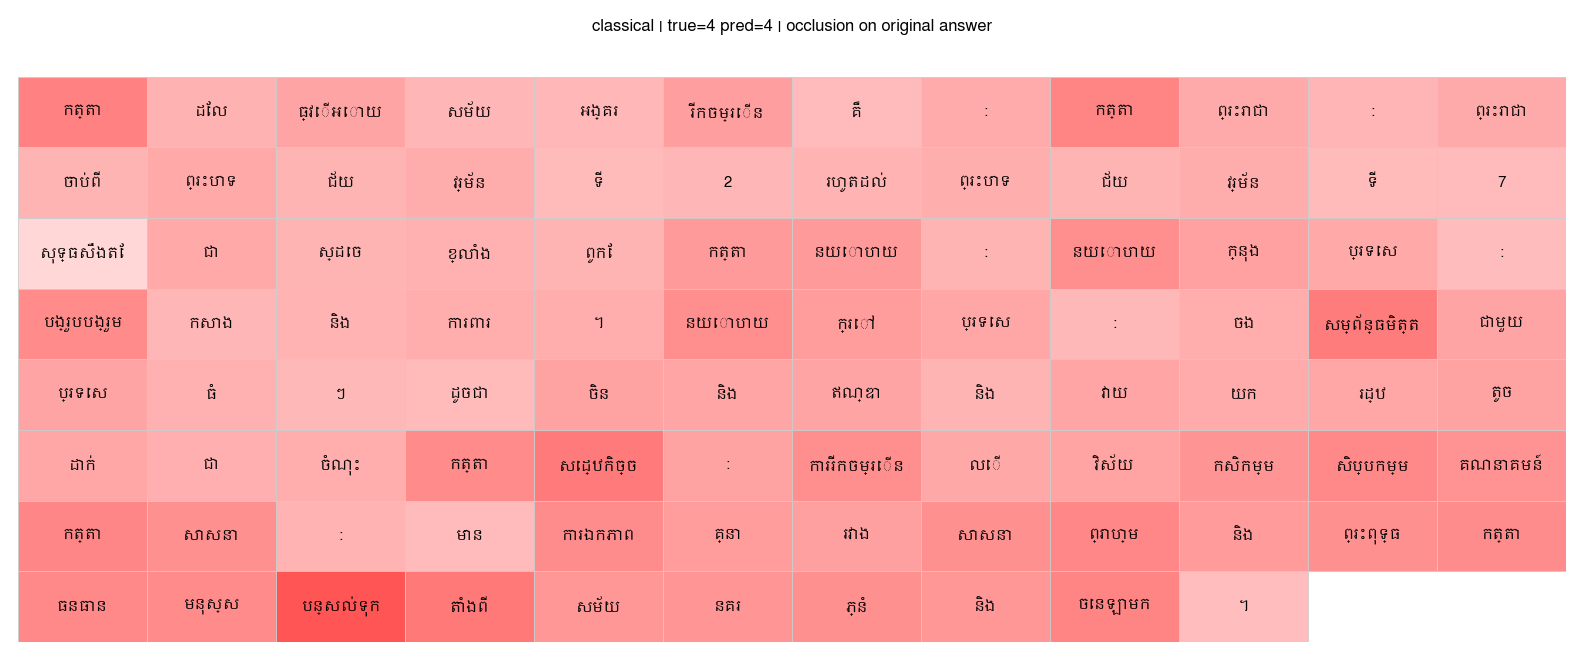
\includegraphics[width=0.95\columnwidth]{figures/heatmap_classical.png}
\caption{Example Khmer word-attribution heatmap (classical, occlusion) on an original student
answer; darker $=$ higher attribution to the predicted score. Rendered with browser text shaping
(from the supplementary HTML), as standard PNG back-ends do not shape Khmer complex script.}
\label{fig:heatmap}
\end{figure}

\section{Discussion}
The ``best model'' is genuinely multi-dimensional, and the three axes behave differently under
scrutiny. On \emph{research} agreement (QWK) the pillars are comparable; on
\emph{deployment} the fine-tuned LLM is the clear winner; on \emph{explainability}, LOO occlusion is the unified method and is reliably faithful for every family. For
accountability-sensitive classroom use,
a 30-second CPU classical model is competitive \emph{and} self-explaining via occlusion; where the
exact teacher score matters, the LLM is preferable. Most importantly, the leakage result is a
cautionary lesson: ASAG benchmarks built on small question pools, ours and much of the
literature, report inflated, seen-question performance; grading genuinely new questions is the
open problem.

\section{Limitations}
\textbf{Single grader:} a second annotator was not available, so we cannot estimate the
human--human ceiling; we report agreement with one teacher and contextualize against the
$0.80$--$0.88$ range reported in the literature, and report results across three dataset variants
as partial mitigation.
\textbf{Scale:} 895--1{,}184 answers and only 41 questions make unseen-question test sets small
and high-variance. \textbf{Completeness:} encoder/LLM unseen-question and faithfulness runs are
ongoing. \textbf{Deployment:} the within-$\pm1$ claim is offline; no classroom field study yet.

\section{Compliance with Ethical Standards}\label{sec:ethics}
This study uses short-answer responses written by school students (minors). \emph{[To be confirmed
by the authors before submission:]} informed consent was obtained from the schools and from
students/guardians for research use and publication of anonymized data, and the study was approved
by~[IRB/ethics body and protocol number], or qualified for exemption because~[reason]. Released
data contain only pseudonymous codes (school/class/student/question identifiers), no names, and
answer text was screened for personally identifying information. The system is intended as a
teacher-assist tool with a human in the loop, not an autonomous high-stakes grader; labels reflect
a single grader and the subject/grade coverage is narrow, so no claim of generalization beyond this
setting is made. The authors declare no conflict of interest.

\section{Conclusion and Future Work}
We presented the first reproducible Khmer ASAG benchmark and an explainability study that measures
faithfulness across model families. The honest picture: pillars are comparable on QWK, the LLM wins
deployment, LOO occlusion is the unified faithful explanation method, and performance collapses on unseen
questions. Future work: complete the encoder/LLM unseen-question and faithfulness runs; enlarge the
question pool to reduce leakage and variance; Khmer continued pretraining; a human study of
explanation quality; and a classroom field deployment. Code, data, seeds, and figures are released
to support reproducibility~\cite{deyoung2020eraser}.

\section*{Acknowledgment}
The authors thank the participating teacher and schools, and the open-source
\texttt{khmer-nltk}~\cite{khmernltk2020}, Unsloth~\cite{unsloth}, and
GTE-multilingual~\cite{gte2024} projects.

\bibliographystyle{IEEEtran}
\bibliography{refs}

\end{document}
